% !TEX root = /home/eb/.vscode/extensions/qftrules.programme-colle/tmp/Exercice.tex
%%%%%%%%%%%%%%%%%%%%%%%%%%%%%%%%%%%%%
\begin{exo}[PC][3][TD]{Induction et freinage magnétique dans un tube conducteur}
  \Notions{\item Moment magnétique \task Induction électromagnétique \task Force de Laplace}
  Un aimant permanent chute dans un tube conducteur de rayon $R$ et d’épaisseur $w \ll R$ négligeable à une vitesse $-v\ez$ dans le référentiel du laboratoire. Dans le référentiel $\mc{R}_A$ de l'aimant, d'origine son centre $\rm A$, et muni d'un repère cylindrique $(r,\theta,z)$, le champ magnétique est de composantes $B_r(r,z)$ et $B_z(r,z)$. Le tube conducteur se déplace à une vitesse $v\ez$ dans ce référentiel.

\begin{fig}[]
  \centering
  
\includegraphics[width=0.35\columnwidth]{chute_aimant.pdf}
  % \capt{Représentation du champ magnétique et des courants de Foucault dans le tube conducteur.}
\end{fig}

\begin{quest}
  % \item Rappeler l’expression du champ magnétostatique dipolaire $\Vec{B}(r,z)$. Dans la suite, on notera simplement $B_r$ et $B_z$ les composantes du champ magnétique sans préciser leurs expressions.

  % \sol{
  % Les composantes du champ magnétique dipolaire $\Vec{B}(\rho,z,t)$ s'obtiennent à partir des formules du cours et de formules de trigonométrie pour exprimer $\cos \theta$ et $\sin \theta$. On trouve
  % % \begin{subequations}
  %   % \eqbox{
  %   $$
  %     % \begin{empheq}[left = \empheqlbrace]{align}
  %       \begin{cases}
  %         B_{r,}(R,z) & = \dfrac{\mu_0 \mathcal{M}}{4 \pi} \dfrac{3 R z}{(r^2 + z^2)^{5/2}}, \label{eq:Brhodip}\\[0.1cm]
  %         B_{z,}(R,z) & = \dfrac{\mu_0 \mathcal{M}}{4 \pi} \dfrac{2 z^2 - R^2}{(R^2 + z^2)^{5/2}},  \label{eq:Brhoz}
  %       \end{cases}
  %         % \end{empheq}
  %     % }
  %     $$
  %     % \end{subequations}
  % }
  \item Le champ magnétostatique induit une f.é.m au sein du tube conducteur en mouvement. De quel type d'induction s'agit-il ? Calculer le flux coupé $\Phi_c$ et en déduire la f.é.m induite $e$.
  \sol{
  La surface coupée par unité de temps vaut 
  $$
  \dd{S}{t} = \dd{h}{t} 2 \pi R = 2v\pi R.
  $$
  On en déduit la f.é.m. 
  \eqbox{
  e = -\dd{\Phi_c}{t} = -2\pi R v B_r.
  }
  }
  \item On admet que cette f.é.m induite est à l'origine d'un courant électrique orthoradial d'intensité élémentaire $\d I = \sigma w E_i \d z$ sur une hauteur $\d z$ de tube, où $\Vec{E_i} = E_i \et$ désigne le champ électrique induit, et $\sigma$ désigne la conductivité électrique du tube. Déterminer la force de Laplace $\d^2\Vec{F}_{a\rightarrow t}$ que le champ magnétique de l'aimant exerce sur une portion du tube conducteur de hauteur $\d z$ et de longueur $\d \ell$. 
  \sol{
    D'après l'expression de la forte de Laplace,
    $$
    \d^2 \Vec{F}_{a\rightarrow t} = \d I \dl \pv \Vec{B} = \beta E_i \d \ell \d z \et \pv (B_r \er + B_z \ez),
    $$
    soit 
    \eqbox{
      \d^2 \Vec{F}_{a\rightarrow t} = \beta E_i \d \ell \d z (-B_r \ez + B_z \er).
    }
  }

  \item En intégrant sur la circonférence du tube, montrer que la force de Laplace que le tube conducteur exerce par unité de hauteur sur l'aimant a pour expression
  $$
  \dd{\F_{t \rightarrow a}}{z} = 2\pi R \sigma w B_r(R,z)^2 v \ez.
  $$
  En déduire que la force de freinage magnétique $\F_{t \rightarrow a}$ que le tube exerce sur l'aimant est proportionnelle à la vitesse $v$ de l'aimant. Expliquer alors l'expérience.
  \sol{
    $$
\dd{\F_{a \rightarrow t}}{z} = \oint \frac{\d^2 \Vec{F}_{a\rightarrow t}}{\d z} = -\beta B_r(R,z) \oint E_i  \d \ell \ez + \beta B_r(R,z) \oint E_i \d \ell \er.
    $$
    Le second terme est nul tandis que $\oint E_i \d \ell = e$. On en déduit 
    $$
    \dd{\F_{a \rightarrow t}}{z}  = -\beta B_r(R,z) e \ez = - \dd{\F_{t \rightarrow a}}{z},
    $$
    en vertu du principe des actions réciproques. Ainsi,
    \eqbox{
      \dd{\F_{t \rightarrow a}}{z} = 2\pi R w \sigma B_r(R,z)^2 v \ez.
    }
    En intégrant sur toute la hauteur $z$ du tube, et en supposant l'aimant loin des bords, on trouve
    $$
    \F_{t \rightarrow a} \simeq \int_{-\infty}^{\infty} 2\pi R \beta B_r(R,z)^2 v \ez \d z = 2\pi R \beta v \int_{-\infty}^{\infty} B_r(R,z)^2 \d z \ez.
    $$
    On trouve alors, avec $\beta  = \sigma w$ et $\sigma$ la conductivité du tube (voir chapitre de conduction), que
    \eqbox{
      \F_{t \rightarrow a} \simeq - \frac{45\mu_0^2 \sigma w \mc{M}^2}{1024R^4} \Vec{v},
    }
    avec $\Vec{v} = -v\ez$ le vecteur vitesse de l'aimant.
    La force de freinage magnétique est donc proportionnelle à la vitesse de l'aimant, comme pour des frottements fluides à bas nombre de Reynolds, en régime laminaire.
  }
\end{quest}
\end{exo}
%%%%%%%%%%%%%%%%%%%%%%%%%%%%%%%%%%%%


%%%%%%%%%%%%%%%%%%%%%%%%%%%%%%%%%%%%%
\begin{exo}[PC][3][TD]{Induction dans un tube conducteur}
  Un aimant chute dans un tube conducteur de rayon $R$ et d’épaisseur $w \ll R$ négligeable. Dans le référentiel $\mc{R}_A$ de l'aimant, muni d'un repère cylindrique $(A,r,\theta,z)$, les composantes du champ magnétique produit par l'aimant sont notées $B_{r,A}(r,z)$ et $B_{z,A}(r,z)$. La composante orthoradiale est nulle. On note $\Vec{B}_A(r,z) = B_{r,A}(r,z) \er + B_{z,A}(r,z) \ez$ le champ magnétique complet.

\begin{fig}[]
  \centering
  
\includegraphics[width=0.4\textwidth]{chute_aimant.pdf}
  \capt{Représentation du champ magnétique et des courants de Foucault dans le tube conducteur.}
\end{fig}

On se place maintenant dans le référentiel $\mc{R}$ du tube conducteur, auquel on attache un autre repère cylindrique $(O,r,\theta,z)$. Dans sa chute verticale, l'altitude de l’aimant dans ce repère est donnée par la fonction du temps $z_0(t)$.
\begin{quest}
  \item Donner l’expression du champ magnétique $\Vec{B}(r,z,t)$ produit par l'aimant dans ce référentiel en fonction de $\Vec{B}_A$ et de $z_0(t)$.

  \sol{
  % Les composantes de $\Vec{B}(\rho,z,t)$ sont
  % \begin{subequations}
  % \begin{empheq}[left = \empheqlbrace]{align}
  %     B_{\rho, \rm dip}(R,z_0-z) & = \dfrac{\mu_0 \mathcal{M}}{4 \pi} \dfrac{3 R (z_0(t)-z)}{(\rho^2 + (z_0(t)-z)^2)^{5/2}}, \label{eq:Brhodip}\$$0.1cm]
  %     B_{z, \rm dip}(R,z_0-z) & = \dfrac{\mu_0 \mathcal{M}}{4 \pi} \dfrac{2 (z_0(t)-z)^2 - R^2}{(R^2 + (z_0(t)-z)^2)^{5/2}},  \label{eq:Brhoz}
  % \end{empheq}\label{eq:champ_dipolaire}
  % \end{subequations}
  }
  \item On note $\Vec{v}=\dd{z_0}{t}\ez$ la vitesse instantanée de l’aimant. Montrer que l'expression du champ électrique suivante :
  $$\Vec{E} = -\Vec{v} \pv \Vec{B}$$ est compatible avec l'équation de Maxwell-Faraday.
  En déduire les composantes de $\Vec{E}(r,z,t)$ en fonction de celles de $\Vec{B}_A(r,z)$.


  \textsc{Données} : $\Rot(\Vec{A} \pv \Vec{B}) = \Vec{A}\, \dive \Vec{B}  - (\Vec{A}\cdot \grad) \Vec{B}$ si $\Vec{A}$
  est un champ uniforme.
  \sol{
  On a
  \begin{align*}
    \dr{B_\rho}{t} = \dd{z_0}{t} \dr{B_\rho}{z_0} = \dfrac{\mu_0 \mathcal{M}}{4 \pi} \dfrac{3 R }{(\rho^2 + (z_0(t)-z)^2)^{5/2}} - \dfrac{5\mu_0 \mathcal{M}}{4 \pi} \dfrac{3 R (z_0(t)-z)^2}{(\rho^2 + (z_0(t)-z)^2)^{7/2}}
  \end{align*}
  }
\end{quest}
On admettra que cette expression du champ électrique, appelée champ électromoteur de Lorentz, est la bonne.

\begin{quest}
  \item Nous verrons que ce champ électrique induit un courant électrique d'intensité élémentaire $\d i = j_s(z,t) \d z$ dans une boucle circulaire $\mc{C}$ du tube conducteur, où $j_s(z,t)$ désigne la densité surface de courant. Ces courants sont appelés courants de Foucault.
  %Cette boucle est donc de rayon $R$ et portée par le vecteur déplacement élémentaire $\Vec{\d \ell} = R \d \theta \et$.
   Calculer la force de Laplace $\d \Vec{F}$ que le champ magnétique exerce sur la tranche de tube conducteur de hauteur $\d z$.
  \sol{
  $$
      \d{\vec{F}} = \oint_\mc{C}  (\d{\Vec{\ell}} \times \Vec{B}) \d{i},
  $$
  donc
  $$
    \d{F} = \d{\Vec{F}} \cdot \ez = \int_{0}^{2\pi} \d{\theta} \, (R \et \times B_r(R,t) \er) \cdot \ez \d{i}= -2 \pi R  B_r(R,z,t) j_s(z,t) \d z.
  $$
  }
  \item En déduire l'expression intégrale de la force de Laplace totale $\Vec{F}$ que le champ magnétique exerce sur le tube, supposé infiniment long, en fonction de $B_r$ et de $j_s$.
  \sol{
  On intègre sur $z$,
  $$
    F = -2 \pi R  \int_{-\infty}^{\infty} B_r(R,z,t) j_s(z,t) \d z.
  $$
  }
\end{quest}
\end{exo}
%%%%%%%%%%%%%%%%%%%%%%%%%%%%%%%%%%%%

%%%%%%%%%%%%%%%%%%%%%%%%%%%%%%%%%%%%%
\begin{exo}[PC][3][TD]{Freinage magnétique dans un tube conducteur}
  On reprend la situation de l’exercice \guill{Induction et freinage magnétique dans un tube conducteur}.
% \ref{Induction dans un tube conducteur}
\begin{quest}
  \question  En utilisant la loi d’Ohm, exprimer la densité surfacique de courant $\j_{\!}s(z,t)$ qui circule dans l’épaisseur du tube conducteur en fonction de $\Vec{E}(R,z,t)$ et $w$.

\sol{
$\j = \sigma \Vec{E}$ donc $\j_s(z,t) = \sigma w E_\theta(R,z,t) \et$.
}
\question En déduire l’expression intégrale de la force de Laplace $\Vec{F}$ en fonction de $\Vec{E}$, puis de $\Vec{B_A}$.

\question On rappelle que dans un repère cylindrique $(A,r,\theta,z)$ centré sur la position $\rm A$ de l’aimant, les composantes du champ magnétique dipolaire s'écrivent
%\begin{subequations}
\begin{empheq}[left = \empheqlbrace]{align}
    B_{r, \rm A}(r,z) & = \dfrac{\mu_0 \mu}{4 \pi} \dfrac{3 r z}{(r^2 + z^2)^{5/2}}, \label{eq:Brhodip}\\[0.1cm]
    B_{z, \rm A}(r,z) & = \dfrac{\mu_0 \mu}{4 \pi} \dfrac{2 z^2 - r^2}{(r^2 + z^2)^{5/2}}.  \label{eq:Brhoz}
\end{empheq}\label{eq:champ_dipolaire}
%\end{subequations}
Montrer que la force de Laplace prend la forme d’une force de frottement linéaire $\Vec{F} = -\alpha \Vec{v}$, où l’on déterminera $\alpha$ en fonction de $R$, $w$, $\sigma$, $\mu$, et $\mu_0$.
\end{quest}

\textsc{Données} : $\int_{-\infty}^{\infty} \frac{x^2}{(x^2+1)^{5/2}} = \frac{\pi}{12}$.
\end{exo}
%%%%%%%%%%%%%%%%%%%%%%%%%%%%%%%%%%%%

%%%%%%%%%%%%%%%%%%%%%%%%%%%%%%%%%%%%%%%%%%%%%%%%%%%%
\begin{exo}[PCSI][2][exp]{Les rails de Laplace}
  \Notions{\item Induction électromagnétique \task Étude énergétique \task Force de Laplace \task Loi des mailles} 
On considère un système de type rails de Laplace, où une barre se déplace sans frottement sur un cadre composé de rails horizontaux parallèles et distants de $\ell$. Cette barre se meut grâce au courant d’intensité $I$ qui circule dans le circuit, généré par une source de résistance interne $R$ qui impose une tension $E_{0}$ constante. On étudie ce système dans le référentiel du cadre, où règne un champ magnétique $\vv{B}=B\,\vv{e_z}$ uniforme et stationnaire. On repère la position de la barre par son abscisse $x$.
%\begin{figure}[h!]
%\centering
\begin{center}

\includegraphics[width=0.4\textwidth]{laplace.pdf}
\end{center}
%\end{figure}
\begin{quest}
\item De quel type d'induction s'agit-il ? Exprimer la fém induite à partir d'un calcul de flux.
%Retrouver l'expression précédente de la fém induite à partir de l'expression du champ électromoteur.
\sol{
  Circuit mobile dans champ stationnaire : \fbox{Lorentz}. Loi de Faraday, avec $e$ dans le sens direct,
  $$
e = -\dd{\Phi}{t},
$$
avec $\Phi = \ell x B$, soit
\eqbox{
  e = -\ell B \dd{x}{t}
}
}
\item Calculer la force de Laplace qui s'exerce sur la tige mobile.
\sol{
Force de laplace
$$
\F = \int I \dl \pv \B = I \left(\int \dl\right) \pv (B \ez) = I (\ell \ey) \pv (B \ez),
$$
soit 
\eqbox{
 \F = I \ell B \ex.
}
}

\item\label{quest:sans_gene} Étude sans générateur. Pour $E_0=0$, déterminer les équations électrique et mécanique, et en déduire une équation sur la vitesse $\dot{x}$. Résoudre en supposant la vitesse initiale égale à $v_0$ et commenter.
\sol{
Il reste à écrire la loi des mailles :
$$
e = RI,
$$
et le PFD :
$$
m \ddd{x}{t} \ex = \F.
$$
Cela donne une équation électrique
$$
\dd{x}{t} + \frac{R}{\ell B}  I= 0,
$$
et une mécanique
$$
\ddd{x}{t} - \frac{\ell B}{m} I = 0.
$$
En isolant le courant : $I = -\frac{\ell B}{R} \dd{x}{t}$, on trouve ensuite
$$
\dd{\dot{x}}{t} + \frac{(\ell B)^2}{mR} \dot{x} = 0.
$$
On peut introduire le temps caractéristique $\tau= \frac{mR}{B^2\ell^2}$. On a alors l’équation
\eqbox{
\dd{\dot{x}}{t} + \frac{\dot{x}}{\tau} = 0.
}
La solution s’écrit $\dot{x}(t) = v_0 e^{-t/\tau}$. Plusieurs remarques.
\begin{liste}
  \item La barre est freinée par la force de Laplace $F_L = - \frac{\dot{x}}{\tau}$ qui agit comme une force de frottement effective. Cela est cohérent avec la loi de modération le Lenz.
  \item Si $v_0=0$, alors $\dot{x}(t)=0$ : la barre reste immobile. Il faut donc un générateur pour mettre la barre en mouvement !
\end{liste}
}
% \item  Découpler ces équations et les résoudre.
\item\label{quest:avec_gene} Étude avec générateur. Reprendre la question précédente pour $E_0$ quelconque.
\sol{
Seule la loi des mailles est modifiée :
$$
e = RI-E_0,
$$

L’intensité du courant vaut alors $I = -\frac{\ell B}{R} \dd{x}{t} + \frac{E_0}{R}$, et on trouve ensuite
$$
\ddd{x}{t} + \frac{(\ell B)^2}{mR} \dd{x}{t} = \frac{\ell B E_0}{m R}.
$$
On peut mettre cette équation sous la forme
\eqbox{
\dd{\dot{x}}{t} + \frac{\dot{x}}{\tau} = \frac{v_{\rm lim}}{\tau}.
}
avec $v_{\rm lim} = \frac{E_0}{B \ell}$. La solution pour une vitesse initiale $v_0$ nulle  vaut
\eqbox{
\dot{x}(t) = v_{\rm lim}(1-e^{-t/\tau}).
}
}
\item Réaliser un bilan de puissance et commenter.
\sol{
  Effectuons un bilan de puissance en l'absence de générateur pour simplifier.
  \begin{enumerate}
    \item D'une part, la puissance totale dissipée est due à l'effet Joule, et a pour expression 
    $$
    \mc{P}_{\rm Joule} = RI^2 = \frac{\ell^2 B^2\dot{x}^2}{R},
    $$
    où l'on a utilisé l'expression de $I$ trouvée dans la \Quest{sans_gene}.
    \item D'autre part, la puissance totale fournie provient de la force de Laplace, soit
    $$
    \mc{P}_{\rm mag} = \Vec{F} \cdot \Vec{v} = I\ell B \dot{x} = -\frac{\ell^2 B^2\dot{x}^2}{R}.
    $$
    On a bien conservation de l'énergie,
    \eqbox{
    \mc{P}_{\rm Joule} + \mc{P}_{\rm mag} = 0.
    }
  \end{enumerate}
  Le résultat reste valable en présence du générateur en ajoutant la puissance électrique fournie,
  $$
  \mc{P}_{\rm elec} = E_0 I,
  $$
  et en remplaçant $I$ par son expression de la \Quest{avec_gene}.
}
\end{quest}
\end{exo}
%%%%%%%%%%%%%%%%%%%%%%%%%%%%%%%%%%%%%%%%%%%%%%%%%%%%%%%%%%

%%%%%%%%%%%%%%%%%%%%%%%%%%%%%%%%%%%%%%%%%%%%%%%%%%%%%%%%%%%%%%
\begin{exo}[PC][2][TD]{Chauffage par induction}
  \Notions{\item Induction de Neuman \task Loi d'Ohm locale \task Effet Joule \task Champ magnétique induit}

  \tcols{0.49}{0.49}{
    Le chauffage par induction est utilisé couramment dans l’industrie (fusion, soudure) et au quotidient (cuisson par induction). On modélise le fond d’une casserole par un cylindre métallique de rayon $a$, de hauteur $h$ et de conductivité $\sigma$ plongé dans un champ magnétique uniforme alternatif $\vec{B}(t)= B_0 \cos(\omega t) \ez$ dirigé selon l'axe du cylindre.
    }
  {
  \begin{center}
  
\includegraphics[scale=1]{tikz_induction_00014.pdf}
  \end{center}
}

\begin{quest}


	\item Par des considérations d’invariance, et en s’aidant d’une équation locale, montrer que loin des bords haut et bas du cylindre le champ électrique est de la forme
	\begin{equation*}
	\E(M,t)= E_{\theta}(r,t) \, \et.
\end{equation*}

	\sol{

	INVARIANCE : Le système est invariant par rotation d'angle $\theta$ autour de $\vec{e}_{z}$ et par translation selon l'axe $Oz$. Le champ électrique ne dépend donc que de la distance
 $r$ à l'axe du cylindre,
$$
  \vec{E} = \vec{E}(r)
$$

SYMÉTRIE : Ici, le champ magnétique (et non pas une distribution de charge) est source du champ électrique, via l'équation de Maxwell-Faraday
$$
  \begin{cases}
   \dfrac{\mathrm{d} E_{z}}{\mathrm{d} r} = 0 \\ \\
   \dfrac{\mathrm{d} r E_{\theta}}{\mathrm{d r}} = - r \dfrac{\mathrm{d} B}{\mathrm{d} t}
  \end{cases}
  \label{eq:far}
$$
Donc $E_z= \text{Cte}$. Par argument énergétique, $E_{z} = E_{r} = 0$ donc $\vec{E} = E_{\theta}(r) \, \vec{e}_{\theta}$.
	}

	\item Calculer ce champ électrique $\vec{E}$ induit par le champ magnétique par deux méthodes différentes.

	 \sol{
\paragraph{Première méthode}
 L'\'Equation \eqref{eq:far} permet le calcul de $\vec{E}$ :

 \begin{equation}
  E_{\theta} = - \frac{1}{2} r \dfrac{\mathrm{d} B}{\mathrm{d t}} + cste
 \end{equation}
 On annule la constante par argument énergétique.

 \begin{equation}
  \vec{E} = - \frac{1}{2} r \dfrac{\mathrm{d} B}{\mathrm{d t}} \, \vec{e}_{\theta} \label{eq:cylrep}
 \end{equation}

 \paragraph{Deuxième méthode} On peut également utiliser le théorème de Stokes en calculant la circulation du champ $\vec{E}$ sur le cercle $\mathcal{C}$ de rayon $r$.

  \begin{minipage}[c][5cm][c]{0.5\textwidth}
    \begin{eqnarray*}
 \oint_{\mathcal{C}} \vec{E}\cdot\vec{dl} & = & \iint_{S} \rot{E}\cdot\vec{dS}\\
						& = & - \iint_{S} \dfrac{\mathrm{d} \vec{B}}{\mathrm{d t}}\cdot\vec{dS} \\
	\mathrm{donc} \qquad 2\pi r E_{\theta} & = & - \pi r^{2} \dfrac{\mathrm{d} B}{\mathrm{d t}} \\
	\mathrm{d'où} \qquad \vec{E} & = & - \frac{1}{2} r \dfrac{\mathrm{d} B}{\mathrm{d t}} \, \vec{e}_{\theta}
    \end{eqnarray*}
  \end{minipage}
  }

	\item Calculer la puissance volumique $p_{\rm vol}$ dissipée par effet Joule, puis la puissance totale $\mc{P}$ dissipée dans le cylindre, ainsi que la moyenne temporelle $\moy{\mc{P}}$. \AN~pour l’aluminium, de conductivité $\sigma = \SI{3.8e7}{S.m^{-1}}$, et un cylindre de rayon $a=\SI{10}{cm}$.

	\sol{La puissance $\mathrm{d}P$ dissipée par effet Joule par un volume $\mathrm{d}\tau$ est donnée par

 \begin{equation*}
 \mathrm{dP} = \vec{j}\cdot\vec{E}\,\mathrm{d}\tau
 \end{equation*}
 où $\vec{j} = \gamma \vec{E}$ est le vecteur densité de courant pour un conducteur. Intégrons sur une couronne de cyllindre d'axe $Oz$ et de rayon $r$ :

 \begin{eqnarray*}
  P & = & \int_{0}^{a} \frac{1}{4} \gamma r^{2} \left(\dfrac{\mathrm{d} B}{\mathrm{d t}}\right)^{2} 2\pi h r \mathrm{dr} \\
    & = & \frac{\pi \gamma a^{4} h}{8} \left(\dfrac{\mathrm{d} B}{\mathrm{d t}}\right)^{2}
 \end{eqnarray*}
	}

	\item Les courants de Foucault induits dans le conducteur génèrent à leur tour un champ magnétique~$B_{\rm i}$. Déterminer ce champ et le comparer à $B_0$ pour une pulsation $\omega = \SI{e3}{rad.s^{-1}}$.

	\sol{
	Le courant est orthoradiale et ne dépend que de $r$ donc $\vec{B}_{\rm in}$ est porté par $\vec{e_z}$ et ne dépend que de $r$,
	$$
	\vec{B}_{\rm in} = B_{\rm in}(r) \vec{e_z}
	$$
	Maxwell-Ampère
	$$
	\rot{B} = \mu_0 \vec{j} = -\dfrac{1}{2}\mu_0 \gamma r \dfrac{\d B}{\d t} \vec{e_\theta} =  \dfrac{1}{r} \dfrac{\d (rB_{\rm in})}{\d r}.
	$$
	et donc
	$$
	B_{\rm in} = -\dfrac{1}{6} \mu_0 \gamma r^2 \dfrac{\d B}{\d t}.
	$$
	Non uniforme, dans le sens opposé à la croissance de $\vec{B}$. Si $\omega$ est la pulsation typique de $\vec{B}$, alors
	$$
	\left| \dfrac{B_{\rm in}}{B} \right| \simeq \mu_0 \gamma a^2 \omega.
	$$
	}


\end{quest}

\textsc{Données :} Opérateur rotationnel en coordonnées cylindriques :

 \begin{equation*}
  \rot{A} =  \left[\frac{1}{r} \frac{\partial A_{z}}{\partial \theta} - \frac{\partial A_{\theta}}{\partial z}\right]   \er +
				   \left[\frac{\partial A_{r}}{\partial z} - \frac{\partial A_{z}}{\partial r}\right]   \et +
				   \left[\frac{1}{r} \frac{\partial (rA_{\theta})}{\partial r} - \frac{1}{r} \frac{\partial A_{r}}{\partial \theta}\right] \ez.
 \end{equation*}

\end{exo}
%%%%%%%%%%%%%%%%%%%%%%%%%%%%%%%%%%%%%%%%%%%%%%%%%%%%%%%%%%%%%%%%%%%%%%%%%%%%%%%%%%%%%%%%%%

%%%%%%%%%%%%%%%%%%%%%%%%%%%%%%%%%%%
\begin{exo}[PC][1][colle]{Induction de Lorentz}
  \Notions{\item Induction électromagnétique}
  Soit un fil conducteur rigide et fermé $\Gamma$ se déplaçant à la vitesse $\Vec{v}$ dans le référentiel $\mc{R}$ du laboratoire, où règne un champ magnétostatique $\Vec{B}(M)$. Le champ électrique est nul dans ce référentiel.
  \begin{quest}
    \item	Donner l'expression de la force de Lorentz $\F_{\rm L}$ sur un porteur de charge $q$ dans le conducteur. On définit la f.é.m $e$ comme le travail par unité de charge de la force de Lorentz sur un tour complet du fil. Montrer que 
    $$
    e = \oint_\Gamma (\Vec{v} \pv \B) \cdot \dl.
    $$
    Quelle est l'unité de $e$ ?
    \sol{
    La force de Lorentz est $\Vec{F}_{\rm L} = q \Vec{v} \pv \Vec{B}$. Notons $\Gamma$ le contour fermé du fil. La f.é.m est le travail par unité de charge de cette force, soit
      $$
      e  = \frac{W_\Gamma}{q} = \frac{1}{q} \oint_\Gamma \Vec{F}_{\rm L} \cdot \d l = \oint_\Gamma (\Vec{v} \pv \B) \cdot \d l,
      $$
    d'où le résultat.
    }
    \item Pendant une durée infiniment petite $\d t$, une portion élémentaire $\dl$ du fil conducteur se déplace d'un vecteur $\Vec{\d r}$. Comment interpréter le vecteur $\Vec{\d r} \pv \dl$ ? Faire un schéma.
    \sol{
    Le vecteur $\Vec{\d r}  \pv \dl$ représente le vecteur de surface élémentaire $\d^2 \Vec{S}_c$ de la surface balayée par le fil pendant la durée $\d t$. La surface $\d^2 S_c$ représente la surface coupée par la portion $\dl$ du fil pendant la durée $\d t$.
    \begin{fig}[label]
      \centering
      % \includegraphics[width=0.3\columnwidth]{flux_coupe.png}
      %\capt{}
    \end{fig}
    }
    \item Montrer alors que la f.é.m $e$ s'écrit également
    $$
    e = -\dd{\Phi_c}{t},
    $$
    où $\Phi_c$ est le flux magnétique coupé par le fil en mouvement. Quel est le nom de cette loi ?
    \sol{
      On utilise la cylicité du produit mixte,
      $$
      e = \oint_\Gamma (\Vec{v} \pv \B) \cdot \dl = \oint_\Gamma (\dl \pv \Vec{v}) \cdot \B = \oint_\Gamma (\dl \pv \dd{\Vec{r}}{t}) \cdot \B = \dd{}{t} \oint_\Gamma (-\d \Vec{S}_c) \cdot \B,
      $$
      soit 
      \eqbox{
        e = -\dd{\Phi_c}{t}.
      }
      Il s'agit de la loi de \fbox{Faraday} de l'induction.
    }
  \end{quest} 

\end{exo}
%%%%%%%%%%%%%%%%%%%%%%%%%%%%%%%%%%%


%%%%%%%%%%%%%%%%%%%%%%%%%%%%%%%%%%%
\begin{exo}[PC][1][colle]{Le disque de Faraday}
  \Notions{\item Induction électromagnétique }
  Un disque conducteur de rayon $R$ tourne à la vitesse angulaire $\omega$ constante autour de son axe, dans un champ magnétique stationnaire et uniforme $\Vec{B} = B \ez$. On ferme le circuit entre le centre du disque en O et un point de contact A au bord du disque. On observe alors la circulation d'un courant électrique dans le circuit.
  \begin{fig}[label]
    \centering
    
\includegraphics[width=0.4\columnwidth]{disque_faraday.png}
    %\capt{}
  \end{fig}
  \begin{quest}
    \item	Quel phénomène est à l'origine de l'apparition de ce courant ? De quel type d'induction s'agit-il ?
     \sol{
    Il s'agit de l'\fbox{induction de Lorentz}.
    }
    \item Déterminer le flux $\d \Phi_c$ coupé  par le disque en rotation pendant une durée $\d t$. En déduire l'expression de la f.é.m induite $e$.
    \sol{
      Un point $M$ du disque se déplace dans la direction orthoradiale à la vitesse angulaire $\omega$. Le vecteur surface coupée élémentaire vaut 
      $$
      \d^2 \Vec{S}_c = \Vec{\d r} \pv \dl = r \omega \d t \et \pv (\d r \er + r \d \theta \et) = -\omega r\d r \d t \ez.
      $$
      En intégrant sur le rayon du disque, on trouve 
      $$\d S_c  = -\frac{R^2}{2} \omega \d t\ez.$$
      Le champ magnétique est uniforme et donc 
      \eqbox{
      \d \Phi_c = \Vec{B} \cdot \Vec{\d S_c} = -\frac{R^2}{2} B \omega \d t.
      }
      On en déduit la f.é.m 
      \eqbox{
      e = -\dd{\Phi_c}{t} = \frac{R^2}{2} B \omega.
      }
    }
  \end{quest}
\end{exo}
%%%%%%%%%%%%%%%%%%%%%%%%%%%%%%%%%%%

%%%%%%%%%%%%%%%%%%%%%%%%%%%%%%%%%%%%%%%%%%%%%%%%%%%%%%%%%%%%%%
\begin{exo}[PT][1][TD]{Induction dans un cylindre métallique}
Un cylindre métallique de rayon $a$, de hauteur $h$ et de conductivité $\gamma$ est plongé dans un champ magnétique uniforme $\vec{B}(t)$ dirigé selon l'axe du cylindre.


  \begin{center}

\includegraphics[scale=0.4]{Cyllindre.eps}
\end{center}

\begin{quest}


	\item En utilisant une équation locale, montrer que loin des bords haut et bas du cylindre le champ électrique est de la forme
	\begin{equation}
	\vec{E} = E_{\theta}(r,t) \, \vec{e_\theta}.
	\end{equation}

	\sol{

	INVARIANCE : Le système est invariant par rotation d'angle $\theta$ autour de $\vec{e}_{z}$ et par translation selon l'axe $Oz$. Le champ électrique ne dépend donc que de la distance
 $r$ à l'axe du cylindre,
$$
  \vec{E} = \vec{E}(r)
$$

SYMÉTRIE : Ici, le champ magnétique (et non pas une distribution de charge) est source du champ électrique, via l'équation de Maxwell-Faraday
$$
  \begin{cases}
   \dfrac{\mathrm{d} E_{z}}{\mathrm{d} r} = 0 \\ \\
   \dfrac{\mathrm{d} r E_{\theta}}{\mathrm{d r}} = - r \dfrac{\mathrm{d} B}{\mathrm{d} t}
  \end{cases}
  \label{eq:far}
$$
Donc $E_z= \text{Cte}$. Par argument énergétique, $E_{z} = E_{r} = 0$ donc $\vec{E} = E_{\theta}(r) \, \vec{e}_{\theta}$.
	}

	\item Calculer le champ électrique $\vec{E}$ induit par le champ magnétique par deux méthodes différentes.

	 \sol{
\paragraph{Première méthode}
 L'\'Equation \eqref{eq:far} permet le calcul de $\vec{E}$ :

 \begin{equation}
  E_{\theta} = - \frac{1}{2} r \dfrac{\mathrm{d} B}{\mathrm{d t}} + cste
 \end{equation}
 On annule la constante par argument énergétique.

 \begin{equation}
  \vec{E} = - \frac{1}{2} r \dfrac{\mathrm{d} B}{\mathrm{d t}} \, \vec{e}_{\theta} \label{eq:cylrep}
 \end{equation}

 \paragraph{Deuxième méthode} On peut également utiliser le théorème de Stokes en calculant la circulation du champ $\vec{E}$ sur le cercle $\mathcal{C}$ de rayon $r$.

  \begin{minipage}[c][5cm][c]{0.5\textwidth}
    \begin{eqnarray*}
 \oint_{\mathcal{C}} \vec{E}\cdot\vec{dl} & = & \iint_{S} \rot{E}\cdot\vec{dS}\\
						& = & - \iint_{S} \dfrac{\mathrm{d} \vec{B}}{\mathrm{d t}}\cdot\vec{dS} \\
	\mathrm{donc} \qquad 2\pi r E_{\theta} & = & - \pi r^{2} \dfrac{\mathrm{d} B}{\mathrm{d t}} \\
	\mathrm{d'où} \qquad \vec{E} & = & - \frac{1}{2} r \dfrac{\mathrm{d} B}{\mathrm{d t}} \, \vec{e}_{\theta}
    \end{eqnarray*}
  \end{minipage}
  }

	\item Calculer la puissance totale dissipée par effet Joule.

	\sol{La puissance $\mathrm{d}P$ dissipée par effet Joule par un volume $\mathrm{d}\tau$ est donnée par

 \begin{equation*}
 \mathrm{dP} = \vec{j}\cdot\vec{E}\,\mathrm{d}\tau
 \end{equation*}
 où $\vec{j} = \gamma \vec{E}$ est le vecteur densité de courant pour un conducteur. Intégrons sur une couronne de cyllindre d'axe $Oz$ et de rayon $r$ :

 \begin{eqnarray*}
  P & = & \int_{0}^{a} \frac{1}{4} \gamma r^{2} \left(\dfrac{\mathrm{d} B}{\mathrm{d t}}\right)^{2} 2\pi h r \mathrm{dr} \\
    & = & \frac{\pi \gamma a^{4} h}{8} \left(\dfrac{\mathrm{d} B}{\mathrm{d t}}\right)^{2}
 \end{eqnarray*}
	}

	\item Les courants de Foucault induits dans le conducteur par effet Joule génèrent à leur tour un champ magnétique~$\vec{B}_{\rm in}$. Déterminer $\vec{B}_{\rm in}$ par la méthode de votre choix et le comparer à $\vec{B}$ pour $a=\SI{5}{cm}$, $\gamma = \SI{6.0e7}{S.m^{-1}}$ et une pulsation typique du champ magnétique $\omega = \SI{1e3}{rad.s^{-1}}$.

	\sol{
	Le courant est orthoradiale et ne dépend que de $r$ donc $\vec{B}_{\rm in}$ est porté par $\vec{e_z}$ et ne dépend que de $r$,
	$$
	\vec{B}_{\rm in} = B_{\rm in}(r) \vec{e_z}
	$$
	Maxwell-Ampère
	$$
	\rot{B} = \mu_0 \vec{j} = -\dfrac{1}{2}\mu_0 \gamma r \dfrac{\d B}{\d t} \vec{e_\theta} =  \dfrac{1}{r} \dfrac{\d (rB_{\rm in})}{\d r}.
	$$
	et donc
	$$
	B_{\rm in} = -\dfrac{1}{6} \mu_0 \gamma r^2 \dfrac{\d B}{\d t}.
	$$
	Non uniforme, dans le sens opposé à la croissance de $\vec{B}$. Si $\omega$ est la pulsation typique de $\vec{B}$, alors
	$$
	\left| \dfrac{B_{\rm in}}{B} \right| \simeq \mu_0 \gamma a^2 \omega.
	$$
	}


\end{quest}

\textsc{Données :} Opérateur rotationnel en coordonnées cylindriques

 \begin{equation}
  \rot{A} =  \left[\frac{1}{r} \frac{\partial A_{z}}{\partial \theta} - \frac{\partial A_{\theta}}{\partial z}\right]   \vec{e_r} +
				   \left[\frac{\partial A_{r}}{\partial z} - \frac{\partial A_{z}}{\partial r}\right]   \vec{e_\theta} +
				   \left[\frac{1}{r} \frac{\partial (rA_{\theta})}{\partial r} - \frac{1}{r} \frac{\partial A_{r}}{\partial \theta}\right]   \vec{e_z}
 \end{equation}

\end{exo}
%%%%%%%%%%%%%%%%%%%%%%%%%%%%%%%%%%%%%%%%%%%%%%%%%%%%%%%%%%%%%%%%%%%%%%%%%%%%%%%%%%%%%%%%%%

%%%%%%%%%%%%%%%%%%%%%%%%%%%%%%%%%%%%%%%%%%%%%%%%%%%%%%%%%%%%%%%%%%%%%%%%%%%%%%%%%%%%%%%%%%
\begin{exo}[PC][1]{Deux rails de Laplace}%{1}
Deux rails de Laplace glissent sans frottement selon la direction $\vv{e_x}$ sur deux rails conducteurs. On note $R$ la résistance équivalente du circuit fermé entre les deux rails, et on négligera son inductance propre. L'ensemble est placé dans un champ magnétique stationnaire uniforme $\vv{B}=B\,\vv{e_z}$. Initialement les deux rails sont en $x_1(0)=x_2(0)=0$. Puis à $t=0$, un opérateur tire le rail 1 par une force extérieure $\vv{F}$ dirigée selon $\vv{e_x}$ qui met le rail 1 en mouvement rectiligne à la vitesse uniforme $v_0\,\vv{e_x}$.
%\begin{figure}[h!]
%\centering
\begin{center}

\includegraphics[width=0.4\textwidth]{laplace_2rails.pdf}
\end{center}
%\end{figure}
\begin{quest}
\item Expliquer qualitativement pourquoi le rail 2 se met aussi en mouvement.
\item Déterminer la loi d'évolution de $x_2(t)$, puis commenter par rapport à la loi de Lenz.
\item Établir par un bilan énergétique l'expression de la puissance extérieure développée par la force qui met en mouvement le rail 1. Commenter.
\end{quest}
\end{exo}
%%%%%%%%%%%%%%%%%%%%%%%%%%%%%%%%%%%%%%%%%%%%%%%%%%%%%%%%%%%%%%%%%%%%%%%%%%%%%%%%%%%%%%%%%%

%%%%%%%%%%%%%%%%%%%%%%%%%%%%%%%%%%%%%%%%%%%%%%%%%%%%%%%%%%%%%%%%%%%%%%%%%
\begin{exo}[PC][1][TD]{Pince ampérométrique}%{1}
Une pince ampérométrique est un instrument de mesure de courants intenses (plusieurs milliers d'Ampère) dont le fonctionnement repose sur l'induction à travers une bobine torique. La bobine torique est constituée de $N$ spires jointives de section rectangulaire. Soit $(Oz)$ l'axe de la bobine. La bobine est de hauteur $h$, de rayon interne $a$ et de rayon externe $b$. On introduit la base des coordonnées cylindriques $(\vec{e_r}, \vec{e_{\theta}}, \vec{e_z})$.

%\begin{figure}[h!]
\begin{center}
%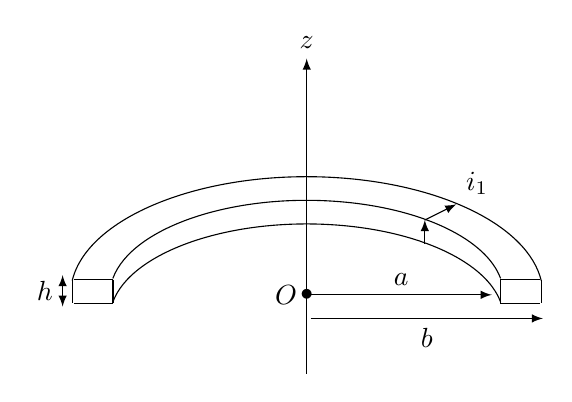
\begin{tikzpicture}

%arc d'ellipse
\tikzset{
    partial ellipse/.style args={#1:#2:#3}{
        insert path={+ (#1:#3) arc (#1:#2:#3)}
    }
}

\draw[->,>=latex] (0,-1) --++(0,4) node[above] {$z$};
\draw (0,0) [partial ellipse=173:7:3cm and 1.5cm];
\draw (0,0) [partial ellipse=170:10:2.5cm and 1.2cm];
\draw (0,-0.3) [partial ellipse=170:10:2.5cm and 1.2cm];
\draw (2.46,0.19) --++(0,-0.3);
\draw (2.98,0.19) --++(0,-0.3);
\draw (-2.46,0.19) --++(0,-0.3);
\draw (-2.98,0.19) --++(0,-0.3);
\draw (2.46,0.19) --++(0.5,0);
\draw (2.46,-0.11) --++(0.5,0);
\draw (-2.46,0.19) --++(-0.5,0);
\draw (-2.46,-0.11) --++(-0.5,0);

\draw[->,>=latex] (0.05,0) --++(2.3,0) node[midway, above]{$a$};
\draw[->,>=latex] (0.05,-0.3) --++(2.95,0) node[midway, below]{$b$};

\draw[<->,>=latex] (-3.1,-0.15) --++(0,0.4) node[midway, left]{$h$};

\draw[->,>=latex] (1.5,0.65) --++(0,0.3);
\draw[->,>=latex] (1.5,0.95) --++(0.4,0.2) node[above right] {$i_1$};
\node at (0,0) {\small $\bullet$};
\node[left] at (0,0) {$O$};

\end{tikzpicture}

\includegraphics[scale=1]{pince.pdf}
\end{center}
%\caption{Coupe d'une pince ampérométrique dans un plan d'axe $(Oz)$. La bobine forme un tore de section rectangulaire de rayons interne $a$ et externe $b$ et de hauteur $h$. Le courant $i_1$ qui parcourt l'enroulement est orienté dans le sens trigonométrique.}
%\label{fig:pince}
%\end{figure}

\begin{quest}
\item On se propose en premier lieu de déterminer l'inductance propre de la bobine. Pour ce faire, un courant $i_1$ est imposé dans l'enroulement comme sur la Fig.~\ref{fig:pince}. Déterminer l'expression du champ magnétique $\vec{B_1}$ à l'intérieur de la bobine.
\item Calculer ensuite le flux de $\vec{B_1}$ à travers les $N$ spires, noté $\Phi_p$, et en déduire l'auto-inductance
\begin{equation}
L_1 = \frac{\mu_0 N^2 h}{2 \pi} \ln\left(\frac{b}{a} \right).
\end{equation}
\item Le courant $i_1$ est coupé et un courant $i_2$ parcourt maintenant l'axe $(Oz)$. Calculer le champ magnétique $\vec{B_2}$ créé par cette distribution de courant puis en déduire l'inductance mutuelle
\begin{equation*}
M =  \frac{\mu_0 N h}{2 \pi} \ln\left(\frac{b}{a} \right).
\end{equation*}

\item Un courant sinusoïdal $i_2(t)=I_2 e^{i\omega t}$ parcourt l'axe $(Oz)$. Soit $i_1(t)=I_1 e^{i\omega t +\phi}$ le courant induit par $i_2$ dans l'enroulement de la bobine. On suppose que la bobine est de résistance nulle (elle est assimilable à un fil). Que vaut la force électromotrice d'induction $e_1$? Montrer que le déphasage vaut $\phi = \pi$ et que
\begin{equation}
I_1 = \frac{I_2}{N}
\end{equation}

\item On prend en compte la résistance $R$ de l'enroulement. Déterminer l'expression de $I_1(\omega)$ et de $\phi(\omega)$.
\end{quest}
\end{exo}
%%%%%%%%%%%%%%%%%%%%%%%%%%%%%%%%%%%%%%%%%%%%%%%%%%%%%%%%%%%%%%%%%%%%%%%%%


%%%%%%%%%%%%%%%%%%%%%%%%%%%%%%%%%%%
\begin{exo}[PC][1][oral]{Allumage d'une lampe par induction}
  Une ligne haute tension transporte un courant sinusoïdal de fréquence $f=50 \mathrm{~Hz}$ et de valeur efficace $I=1 \mathrm{kA}$. On approche une bobine plate de $N$ spires carrées de côté $a=30 \mathrm{~cm}$ à une distance $d=2 \mathrm{~cm}$ comme indiqué sur le schéma. Cette bobine, d'inductance propre et de résistance négligeables, est fermée sur une ampoule qui éclaire si la tension efficace à ses bornes est supérieure à $\SI{1.5}{V}$.

\begin{center}

\includegraphics[width=0.4\columnwidth]{2024_05_15_c14ed6583b37c28466fdg-1}
\end{center}

Déterminer le nombre de spires $N$ pour que l'ampoule s'allume dans cette situation.



% Données :

% Perméabilité du vide : $\mu_{0}=4 \pi .10^{-7} \mathrm{H} . \mathrm{m}^{-1}$;

% Permitivité du vide : $\varepsilon_{0}=\frac{1}{36 \pi} \cdot 10^{-9} \mathrm{~F} \cdot \mathrm{m}^{-1}$.
\sol{
\section*{Analyse stratégique de l'énoncé}
Il s'agit ici d'un exercice d'électromagnétisme dans lequel le couplage mutuel par induction entre deux circuits magnétiques doit être étudié.

\begin{enumerate}
  \item Pour calculer le coefficient d'inductance mutuelle $M$ entre deux circuits magnétiques, il est nécessaire de calculer le flux magnétique entre ces deux circuits. Il faudra en particulier tenir compte des $N$ spires qui constituent la bobine. Pour éviter les erreurs, les orientations des circuits et des champs magnétiques doivent apparaître sur un schéma précisément annoté.
\end{enumerate}

Rapport du jury 2013

Il y a de nombreuses erreurs dans l'évaluation de flux ou de circulations. Celles-ci pourraient être facilement dépistées en définissant par exemple au moyen d'une figure le domaine d'intégration et le choix des éléments de longueur, de surface ou de volume.

Dans cet exercice, le champ magnétique créé par un fil infini autour de lui n'est pas connu, il est donc nécessaire de le déterminer au préalable. Pour ce faire, on\\
doit appliquer le théorème d'Ampère en utilisant les propriétés d'invariance et de symétrie de la distribution de courant.

Rapport du jury 2014

En électrostatique et magnétostatique, les notions de ligne de champ et de tube de champ ainsi que l'application des théorèmes de Gauss ou d'Ampère même dans des cas simples pose souvent problème aux candidats.

\section*{Rapport du jury 2011}
Les arguments de symétrie sont trop souvent oubliés ou confondus avec les propriétés d'invariance. Nous soulignons encore la nécessité de rigueur concernant les signes; les surfaces, les contours et leurs orientations doivent toujours être clairement définis.

$\hookrightarrow$ Le coefficient d'inductance mutuelle $M$ entre les deux circuits magnétiques doit être déterminé en calculant le flux du champ magnétique créé par la ligne à haute tension dans la bobine constituée de $N$ spires.

\begin{enumerate}
  \setcounter{enumi}{1}
  \item Pour répondre à cette question il est nécessaire de tenir compte du phénomène d'induction électromagnétique et en particulier de la force électromotrice d'induction $e$ qui apparaît aux bornes de la bobine. Cette tension $e$ fera briller l'ampoule si sa valeur efficace est supérieure à $1,5 \mathrm{~V}$. Pour évaluer $e$, il faut appliquer la loi de Lenz-Faraday en étant particulièrement vigilant aux signes des grandeurs physiques utilisées. La f.e.m. d'induction $e$ dépendra du nombre de spires $N$ de la bobine.
\end{enumerate}

Rapport du jury 2013

En induction électromagnétique, il est généralement nécessaire d'effectuer des schémas électrique ou mécanique équivalents, avec une définition de I'orientation des conducteurs, de la f.e.m. induite ou un bilan des forces sur lequel figure la force de Laplace.

Rapport du jury 2012

En électromagnétisme, il y a toujours des problèmes de signe sur les exercices d'induction électromagnétique.

$\hookrightarrow$ Pour déterminer le nombre $N$ de spires de la bobine nécessaire pour faire briller l'ampoule, il faut déterminer la f.e.m. d'induction $e$ aux bornes de la bobine à l'aide de la loi de Lenz-Faraday.

\section*{Corrigé}
\begin{enumerate}
  \item On note (1), la ligne haute tension (circuit 1) et (2), la bobine (circuit 2).
\end{enumerate}

Pour déterminer $\overrightarrow{B_{1}}$, le champ magnétique créé par la ligne à haute tension, on doit dans un premier temps déterminer la valeur du champ magnétique créé par un fil infini parcouru par un courant $i(t)$. Pour ce faire on va appliquer le théorème d'Ampère.

Rapport du jury 2014

En électrostatique et magnétostatique, les notions de ligne de champ et de tube de champ ainsi que l'application des théorèmes de Gauss ou d'Ampère même dans des cas simples pose souvent problème aux candidats.

On adopte le système de coordonnées cylindriques.

Rapport du jury 2011

Les arguments de symétrie sont trop souvent oubliés ou confondus avec les propriétés d'invariance. Nous soulignons encore la nécessité de rigueur concernant les signes; les surfaces, les contours et leurs orientations doivent toujours être clairement définis.

\begin{itemize}
  \item Invariance de la distribution de courants par translation suivant $O z$ et par rotation autour de $O z$, d'où $B(r, \theta, z)=B(r)$.
\end{itemize}

Le plan $M O z$ est plan de symétrie de la distribution de courants donc $\vec{B}(M)$ est normal à ce plan.

Le plan normal à $O z$ et contenant $M$ est plan d'antisymétrie de la distribution de courants donc $\vec{B}(M)$ est dans ce plan.

Conclusion : $\vec{B}=B(r) \cdot \overrightarrow{e_{\theta}}$.

\begin{center}

\includegraphics[width=\columnwidth]{2024_05_15_c14ed6583b37c28466fdg-3}
\end{center}

\begin{itemize}
  \item Contour d'Ampère $\mathcal{C}$, cercle orienté, passant par $M$ et de rayon $r$.

  \item Application du théorème d'Ampère :

\end{itemize}

$$
\oint_{\mathcal{C}} \vec{B} \cdot \overrightarrow{d \ell}=\oint_{\mathcal{C}} B(r) \cdot \overrightarrow{e_{\theta}} \cdot d \ell \overrightarrow{e_{\theta}}=B(r) \oint_{\mathcal{C}} d \ell=2 \pi r B(r)
$$

Et, $I_{\mathrm{enl}}=I$ donc :

$$
\oint_{\mathcal{C}} \vec{B} \cdot \overrightarrow{d \ell}=\mu_{0} I_{\mathrm{en} 1} \Longleftrightarrow 2 \pi r B(r)=\mu_{0} I \Rightarrow \vec{B}=\frac{\mu_{0} I}{2 \pi r} \overrightarrow{e_{\theta}}
$$

On obtient donc :

$$
\overrightarrow{B_{1}}=\frac{\mu_{0} i(t)}{2 \pi r} \overrightarrow{e_{\theta}}
$$

Pour déterminer l'inductance mutuelle $M$ entre les deux circuits, on doit calculer le flux du circuit (1) dans le circuit (2) constitué de $N$ spires.

$$
\begin{gathered}
\phi_{12}=M_{12} i_{1}=M i_{1}=M i(t) \\
\phi_{12}=N \iint_{S_{2}} \overrightarrow{B_{1}} \cdot \overrightarrow{d S_{2}}
\end{gathered}
$$

En orientant le circuit (2) comme sur le schéma ci-contre, on obtient :

$$
\begin{gathered}
M i(t)=N \iint_{S_{2}} B_{1} \cdot d S_{2} \\
M i(t)=N \iint_{S_{2}} \frac{\mu_{0} i(t)}{2 \pi r} \cdot d S_{2} \\
M I \sqrt{2} \cos (\omega t)=N \int_{S_{2}} \frac{\mu_{0} I \sqrt{2} \cos (\omega t) a d r}{2 \pi r}
\end{gathered}
$$

\begin{center}

\includegraphics[width=\columnwidth]{2024_05_15_c14ed6583b37c28466fdg-4(1)}
\end{center}

\begin{center}

\includegraphics[width=\columnwidth]{2024_05_15_c14ed6583b37c28466fdg-4}
\end{center}

Rapport du jury 2013

Il y a de nombreuses erreurs dans l'évaluation de flux ou de circulations. Celles-ci pourraient être facilement dépistées en définissant par exemple au moyen d'une figure le domaine d'intégration et le choix des éléments de longueur, de surface ou de volume.

On peut donc déduire de cette équation l'inductance mutuelle $M$ entre les deux circuits :

$$
\begin{gathered}
M=N \int_{d}^{d+a} \frac{\mu_{0} a d r}{2 \pi r}=\frac{N \mu_{0} a}{2 \pi}[\ln r]_{d}^{d+a} . \\
M=\frac{N \mu_{0} a}{2 \pi} \ln \left(\frac{d+a}{d}\right)
\end{gathered}
$$

\begin{enumerate}
  \setcounter{enumi}{1}
  \item Le champ magnétique $\overrightarrow{B_{1}}$ créé par la ligne à haute tension va créer un courant induit dans la bobine constituée de $N$ spires. On va donc voir apparaître une force électromotrice (f.e.m.) e d'induction aux bornes de la bobine. L'objectif de cette question est d'évaluer cette f.e.m. d'induction $e$.
\end{enumerate}

Rapport du jury 2012

En électromagnétisme, il y a toujours des problèmes de signe sur les exercices d'induction électromagnétique.

D'après la loi de Lenz-Faraday :

$$
\begin{gathered}
e=-\frac{d \phi}{d t}=-\frac{d}{d t}\left(M i_{1}\right)=-M \frac{d i(t)}{d t} \\
e=-\frac{N \mu_{0} a}{2 \pi} \ln \left(\frac{d+a}{d}\right) \frac{d}{d t}(I \sqrt{2} \cos (\omega t)) \\
e=\frac{N \mu_{0} a}{2 \pi} I \sqrt{2} \omega \ln \left(\frac{d+a}{d}\right) \sin (\omega t)
\end{gathered}
$$

Dans l'énoncé, on indique que l'ampoule éclaire si la tension efficace à ses bornes est supérieure à $1,5 \mathrm{~V}$. On obtient une f.e.m. d'induction de la forme $e=E \sqrt{2} \sin (\omega t)$ avec $E$ la valeur efficace de $e$. Ainsi l'ampoule éclaire si :

$$
\begin{aligned}
E & =\frac{N \mu_{0} a}{2 \pi} I \omega \ln \left(\frac{d+a}{d}\right)>1,5 \mathrm{~V} \\
\Leftrightarrow N>\frac{1,5 \times 2 \pi}{\mu_{0} a I \omega \ln \left(\frac{d+a}{d}\right)} & =\frac{1,5 \times 2 \pi}{4 \pi \cdot 10^{-7} \times 0,3.10^{3} \times 2 \pi \times 50 \times \ln \left(\frac{0,32}{0,02}\right)}=29 \text { spires. }
\end{aligned}
$$

Il faut au minimum une bobine constituée de 29 spires pour que l'ampoule éclaire.

\section*{Techniques à mémoriser}
$\checkmark$ Il faut se souvenir que le choix de l'orientation du circuit est important pour effectuer un raisonnement correct dans un dispositif qui est le siège d'un phénomène d'induction.

Rapport du jury 2012

En électromagnétisme, il y a toujours des problèmes de signe sur les exercices d'induction électromagnétique.

$\triangle$ Il faut se souvenir que pour calculer le flux magnétique entre deux circuits, il faut absolument faire un schéma qui oriente les circuits étudiés et qui fait apparaître les champs magnétiques.

Rapport du jury 2013

Il y a de nombreuses erreurs dans l'évaluation de flux ou de circulations. Celles-ci pourraient être facilement dépistées en définissant par exemple au moyen d'une figure le domaine d'intégration et le choix des éléments de longueur, de surface ou de volume.

$\checkmark$ Il faut se souvenir de la manière dont on détermine le champ magnétique créé par un fil infini autour de lui à l'aide du théorème d'Ampère.

Rapport du jury 2014

En électrostatique et magnétostatique, les notions de ligne de champ et de tube de champ ainsi que l'application des théorèmes de Gauss ou d'Ampère même dans des cas simples pose souvent problème aux candidats.

\section*{Rapport du jury 2011}
Les arguments de symétrie sont trop souvent oubliés ou confondus avec les propriétés d'invariance. Nous soulignons encore la nécessité de rigueur concernant les signes; les surfaces, les contours et leurs orientations doivent toujours être clairement définis.

\section*{Formulaire}
\begin{itemize}
  \item Le phénomène d'induction consiste en l'apparition d'une force électromotrice (f.e.m.) $e$ dite induite et d'un courant induit $i(t)$ dans un circuit électrique soumis à un flux magnétique variable au cours du temps.

  \item On observe un phénomène d'induction magnétique lorsque le flux du champ magnétique $\vec{B}$ à travers un circuit varie au cours du temps :

\end{itemize}

$$
\phi=\iint_{\mathcal{S}} \vec{B} \cdot \overrightarrow{d S}
$$

\begin{itemize}
  \item Loi de Lenz-Faraday :
\end{itemize}

Un circuit traversé par un flux magnétique variable est le siège d'une force électromotrice (f.e.m.) d'induction $e$ telle que :

$$
e=-\frac{d \phi}{d t}
$$

\begin{itemize}
  \item Coefficient d'inductance mutuelle $M$ :
\end{itemize}

Le flux créé par le circuit 1 à travers le circuit 2 a pour expression :

$$
\phi_{12}=\iint_{\mathcal{S}_{2} / \mathcal{C}_{2}} \overrightarrow{B_{1}} \cdot d \overrightarrow{S_{2}}=M_{12} \cdot i_{1}(t)
$$

Le flux créé par le circuit 2 à travers le circuit 1 a pour expression :

$$
\phi_{21}=\iint_{\mathcal{S}_{1} / \mathcal{C}_{1}} \overrightarrow{B_{2}} \cdot d \overrightarrow{S_{1}}=M_{21} \cdot i_{2}(t)
$$

\begin{center}

\includegraphics[width=\columnwidth]{2024_05_15_c14ed6583b37c28466fdg-6}
\end{center}

On note $M$ le coefficient d'inductance mutuelle entre les deux circuits tel que :

$$
M=M_{12}=M_{21} \text { en Henry (H). }
$$
}
\end{exo}
%%%%%%%%%%%%%%%%%%%%%%%%%%%%%%%%%%%